\section{Results}
\label{sec:results}

\subsection{What routing buys, and what it costs}
\label{sec:routing-results}


\begin{table*}[t]
\centering
\caption{Routing-policy performance on the BP3C50ID external split under antigen-level resampling. Intervals are 95\% two-way bootstrap intervals over antigens and seeds (15 antigens, 10 seeds, 2000 resamples), so they carry the uncertainty that matters for a claim about other antigens. Carbon is a model-based estimate, not a metered measurement (Section~\ref{sec:cost-accounting}).}
\label{tab:policy-summary}
\small
\begin{tabular}{lrrrr}
\toprule
Policy & MCC & ROC-AUC & Latency (ms) & Raw-sequence share \\
\midrule
local-only & 0.167 \tiny[0.100, 0.229] & 0.659 \tiny[0.596, 0.712] & 0.4 \tiny[0.4, 0.5] & 0.000 \tiny[0.000, 0.000] \\
edge-only & 0.209 \tiny[0.150, 0.266] & 0.678 \tiny[0.621, 0.726] & 42.4 \tiny[37.2, 48.2] & 1.000 \tiny[1.000, 1.000] \\
adaptive-split & 0.192 \tiny[0.121, 0.255] & 0.673 \tiny[0.611, 0.724] & 13.6 \tiny[4.4, 24.0] & 0.285 \tiny[0.087, 0.507] \\
carbon-guard & 0.165 \tiny[0.091, 0.233] & 0.658 \tiny[0.595, 0.711] & 6.6 \tiny[1.0, 14.5] & 0.133 \tiny[0.013, 0.293] \\
\midrule
PLM local-only & 0.195 \tiny[0.124, 0.259] & 0.678 \tiny[0.614, 0.739] & 29.6 \tiny[17.2, 51.0] & 0.000 \tiny[0.000, 0.000] \\
PLM edge-only & 0.209 \tiny[0.133, 0.280] & 0.691 \tiny[0.623, 0.755] & 68.3 \tiny[54.3, 87.6] & 1.000 \tiny[1.000, 1.000] \\
PLM region-constrained & 0.219 \tiny[0.132, 0.310] & 0.690 \tiny[0.620, 0.760] & 68.3 \tiny[54.3, 87.6] & 1.000 \tiny[1.000, 1.000] \\
PLM adaptive-split & 0.199 \tiny[0.124, 0.268] & 0.680 \tiny[0.615, 0.739] & 47.0 \tiny[29.3, 70.5] & 0.273 \tiny[0.107, 0.473] \\
PLM conformal-guard & 0.199 \tiny[0.124, 0.268] & 0.680 \tiny[0.615, 0.739] & 47.0 \tiny[29.3, 70.5] & 0.273 \tiny[0.107, 0.473] \\
\bottomrule
\end{tabular}
\end{table*}

\begin{table*}[t]
\centering
\caption{Paired differences between routing policies under antigen-level resampling, with 95\% two-way bootstrap intervals. All four quality metrics are shown for every comparison. An interval containing zero is reported as no detected difference; intervals excluding zero are marked $^{\ast}$.}
\label{tab:paired}
\small
\setlength{\tabcolsep}{4pt}
\begin{tabular}{@{}lrrrr@{}}
\toprule
Comparison & $\Delta$MCC & $\Delta$ROC-AUC & $\Delta$AP & $\Delta$F1 \\
\midrule
adaptive-split vs edge-only & -0.017 & -0.005 & -0.005 & +0.002 \\
 & \tiny[-0.066, +0.026] & \tiny[-0.040, +0.021] & \tiny[-0.029, +0.027] & \tiny[-0.030, +0.034] \\
\addlinespace
adaptive-split vs local-only & +0.025 & +0.014 & +0.015 & +0.033$^{\ast}$ \\
 & \tiny[-0.011, +0.065] & \tiny[-0.004, +0.038] & \tiny[-0.001, +0.041] & \tiny[+0.004, +0.075] \\
\addlinespace
carbon-guard vs adaptive-split & -0.027$^{\ast}$ & -0.015 & -0.015$^{\ast}$ & -0.016$^{\ast}$ \\
 & \tiny[-0.064, -0.001] & \tiny[-0.038, +0.000] & \tiny[-0.040, -0.000] & \tiny[-0.039, -0.001] \\
\addlinespace
PLM region-constrained vs PLM local-only & +0.024 & +0.012 & +0.018$^{\ast}$ & +0.014 \\
 & \tiny[-0.024, +0.073] & \tiny[-0.011, +0.033] & \tiny[+0.003, +0.036] & \tiny[-0.020, +0.049] \\
\addlinespace
PLM adaptive-split vs PLM edge-only & -0.010 & -0.011$^{\ast}$ & -0.014$^{\ast}$ & -0.006 \\
 & \tiny[-0.038, +0.016] & \tiny[-0.022, -0.001] & \tiny[-0.026, -0.005] & \tiny[-0.027, +0.012] \\
\bottomrule
\end{tabular}
\end{table*}


\begin{figure*}[t]
\centering
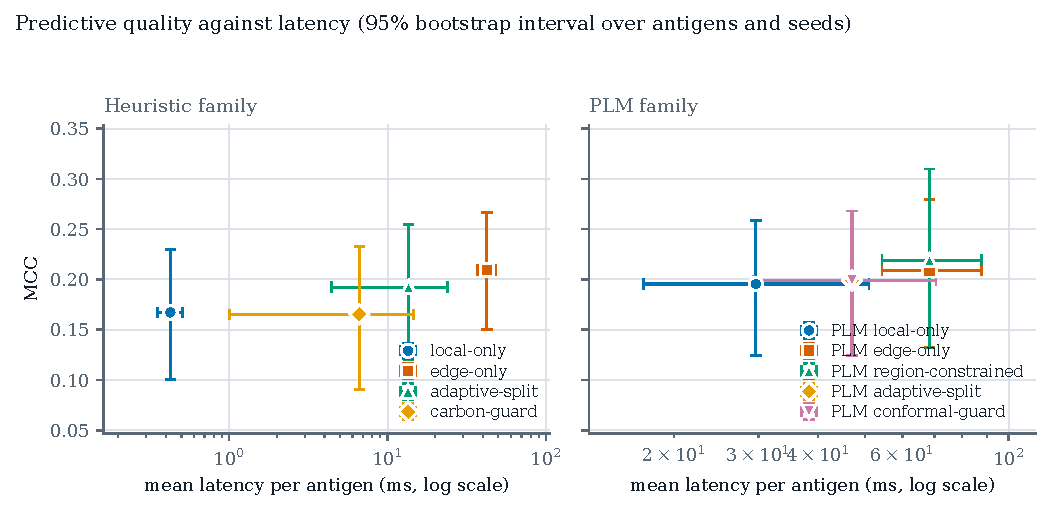
\includegraphics[width=\textwidth]{figures/fig_quality_latency.pdf}
\caption{Predictive quality against mean per-antigen latency on the BP3C50ID
external split, by policy family. Points are means over \NumSeeds{} seeds; bars
are 95\% bootstrap intervals on both axes. In the PLM panel the adaptive-split
and conformal-guard markers coincide exactly, because the conformal criterion
never altered a routing decision on this split.}
\label{fig:quality-latency}
\end{figure*}

\begin{figure*}[t]
\centering
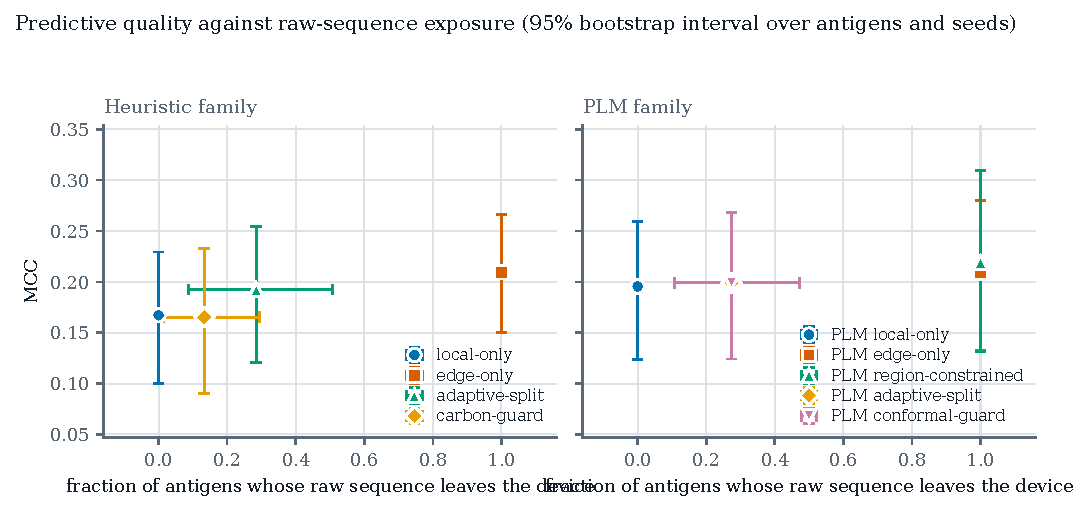
\includegraphics[width=\textwidth]{figures/fig_quality_datamovement.pdf}
\caption{Predictive quality against the fraction of antigens whose raw sequence
is transmitted. Policies at zero on the horizontal axis never transmit;
edge-only transmits every antigen. Adaptive-split occupies the interior of this
trade-off, which always-local and always-remote execution cannot.}
\label{fig:quality-data}
\end{figure*}

Table~\ref{tab:policy-summary} reports every policy on the BP3C50ID external
split across \NumSeeds{} seeds, and Table~\ref{tab:paired} gives the paired
comparisons that the claims below rest on.

Those five comparisons were fixed before the resampling was run: each contrasts
a routing policy with the always-local or always-remote baseline it is meant to
improve on, within its own predictor family. The resampling itself produces
intervals for all \PolicyPairsComputed{} orderable pairs of policies on each
metric, or \QualityIntervalsComputed{} intervals on the four quality metrics
together. We mark intervals that exclude zero in Table~\ref{tab:paired} as a
reading aid for those five rows, and no multiplicity correction is applied. A
reader should not treat the marks as a family-wise claim: across
\QualityIntervalsComputed{} intervals a handful would fall outside zero under
a global null, and several of the marked endpoints sit close enough to zero
that the Monte Carlo error of a \AntigenBootstrapRepeats{}-resample bootstrap
could move them. We draw no conclusion from any single mark, and the
conclusions below rest on the size and direction of the differences rather
than on which intervals happen to exclude zero.

Two points about those intervals before the results. They are two-way
bootstrap intervals over antigens and seeds
(\AntigenBootstrapRepeats{} resamples), not intervals over seeds alone. The
distinction is not cosmetic: the test split holds the same
\AntigenCount{} antigens in every seed, so a seed-only interval measures
how much a number moves when the harness is re-run and says nothing about how
it would move on different antigens. On this data seed-only intervals
are roughly an order of magnitude narrower: local-only MCC is
\ALocalOnlyMcc{} [\ALocalOnlyMccLo{}, \ALocalOnlyMccHi{}] under antigen
resampling against a seed-only width of a hundredth. For two of the
policies the seed-only ROC-AUC interval has width zero, because the underlying
predictor is deterministic and only the validation split moves. Every interval
below is the antigen-level one. We report it this way because the claims are
claims about antigens.

The first result is that the latency and disclosure benefits of routing are
large and survive this resampling, while the quality questions do not resolve
at this sample size. Figure~\ref{fig:quality-latency} plots predictive quality
against mean
per-antigen latency for each policy family.

Against always-remote execution, adaptive-split cuts mean latency by
\(\ADAsVsEoLatency{}\,\)ms [\ADAsVsEoLatencyLo{}, \ADAsVsEoLatencyHi{}] and
reduces the fraction of antigens whose raw sequence is transmitted by
\ADAsVsEoRawShare{} [\ADAsVsEoRawShareLo{}, \ADAsVsEoRawShareHi{}]
(Figure~\ref{fig:quality-data} shows quality against that fraction). Neither
difference could have come out positive: a policy that routes some antigens
cannot be slower than one that routes all of them, and cannot transmit more
sequences. These intervals therefore say how large the gain is on other
antigens, not whether there is one. On quality it differs by
\(\Delta\)MCC \ADAsVsEoMcc{} [\ADAsVsEoMccLo{}, \ADAsVsEoMccHi{}],
\(\Delta\)ROC-AUC \ADAsVsEoAuc{} [\ADAsVsEoAucLo{}, \ADAsVsEoAucHi{}],
\(\Delta\)AP \ADAsVsEoAp{} [\ADAsVsEoApLo{}, \ADAsVsEoApHi{}] and \(\Delta\)F1
\ADAsVsEoFOne{} [\ADAsVsEoFOneLo{}, \ADAsVsEoFOneHi{}]. All four contain zero.

We want to be careful about what that does and does not license. It is not a
demonstration of equivalence. With \AntigenCount{} antigens the interval on
\(\Delta\)MCC spans roughly \(\pm 0.05\), so a quality loss large enough to
matter in practice would not be detected here. The defensible statement is that
routing's quality cost relative to always-remote execution is not resolved at
this sample size, while its latency and disclosure benefits are.

The comparison against always-local execution tells the same story from the
other side. \(\Delta\)MCC is \ADAsVsLoMcc{}
[\ADAsVsLoMccLo{}, \ADAsVsLoMccHi{}], \(\Delta\)ROC-AUC \ADAsVsLoAuc{}
[\ADAsVsLoAucLo{}, \ADAsVsLoAucHi{}] and \(\Delta\)AP \ADAsVsLoAp{}
[\ADAsVsLoApLo{}, \ADAsVsLoApHi{}], all containing zero, while
\(\Delta\)F1 is \ADAsVsLoFOne{} [\ADAsVsLoFOneLo{}, \ADAsVsLoFOneHi{}], which
does not. One metric of four separates them. Under seed-only resampling the
same comparison appears decisive on every metric, with \(\Delta\)MCC
\DAsVsLoMcc{} [\DAsVsLoMccLo{}, \DAsVsLoMccHi{}] and a sign test over seeds at
\(p=\SAsVsLoMccP{}\). That sign test is a statement about ten re-runs on fifteen
fixed antigens, and we no longer rest anything on it.

Two comparisons do survive. The carbon-guard policy is worse than adaptive-split
on three of four metrics (\(\Delta\)MCC \ADCgVsAsMcc{}
[\ADCgVsAsMccLo{}, \ADCgVsAsMccHi{}]), so its latency and carbon savings are
bought with quality. Within the PLM family, always-remote execution beats
always-local on ROC-AUC and average precision. PLM routing gives part of
that back (\(\Delta\)ROC-AUC \ADPasVsPeoAuc{}
[\ADPasVsPeoAucLo{}, \ADPasVsPeoAucHi{}] against PLM always-remote): in the
family where the remote model is genuinely stronger, routing's quality cost is
detectable even here.

Table~\ref{tab:scenarios} reports the robustness axes the harness provides. The
informative row is the one where the remote tier is unavailable: every
adaptive-versus-local difference is then exactly zero, because routing degrades
to local-only behaviour rather than failing. The grid-intensity axes move
nothing that matters, and the parameter the carbon results are most sensitive
to --- the embodied amortisation constant --- is not among the available axes
(Section~\ref{sec:limitations}).


\begin{table}[t]
\centering
\caption{Sensitivity of the adaptive-split comparisons to the scenario axes available in the harness. Values are mean $\Delta$MCC over seeds. The grid-intensity axes do not touch predictive quality by construction and are included to show which axes were varied; the remote-tier-unavailable row is the informative one, where routing degrades exactly to always-local behaviour. The dominant carbon parameter, the embodied amortisation constant, is not among the available axes.}
\label{tab:scenarios}
\small
\begin{tabular}{lrr}
\toprule
Scenario & $\Delta$MCC vs local-only & $\Delta$MCC vs edge-only \\
\midrule
baseline & +0.034 & -0.010 \\
remote tier unavailable & +0.000 & +0.000 \\
network $+\SI{50}{\milli\second}$ & +0.034 & -0.010 \\
network $+\SI{5}{\milli\second}$ & +0.034 & -0.010 \\
grid intensity $\times 1.5$ & +0.034 & -0.010 \\
grid intensity $\times 0.5$ & +0.034 & -0.010 \\
\bottomrule
\end{tabular}
\end{table}


\begin{figure*}[t]
\centering
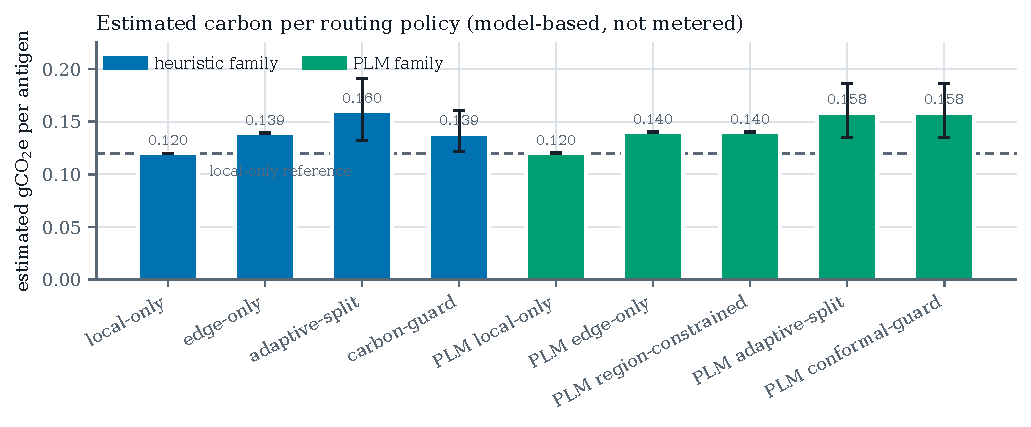
\includegraphics[width=\textwidth]{figures/fig_carbon.pdf}
\caption{Modelled carbon per antigen by policy, with 95\% intervals. These are
outputs of the energy model described in Section~\ref{sec:cost-accounting},
computed from fixed device power, an amortised embodied term and measured
latency; they are not metered measurements. Uncertainty-triggered routing is
the most carbon-intensive policy here because a routed antigen is charged two
device-requests; the ordering is specific to this checkpoint pair and reverses
for a larger remote tier, as the text below sets out.}
\label{fig:carbon}
\end{figure*}

\begin{table}[t]
\centering
\caption{Provenance of each reported cost quantity. Only latency is measured; the energy and carbon figures are derived from fixed device power and a grid-intensity constant, and are therefore model outputs rather than measurements.}
\label{tab:provenance}
\small
\begin{tabular}{ll}
\toprule
Quantity & Provenance \\
\midrule
Latency & timed benchmark execution \\
Energy & estimated from fixed power and latency \\
Operational carbon & estimated from energy and grid intensity \\
Embodied carbon & amortized estimate from device metadata \\
\bottomrule
\end{tabular}
\end{table}


The second result runs against the expectation that motivated the policy.
Figure~\ref{fig:carbon} shows modelled carbon per antigen for every policy.
Adaptive-split is the \emph{highest} of the nine at
\AdaptiveSplitCarbon{}~gCO\textsubscript{2}e
[\AdaptiveSplitCarbonLo{}, \AdaptiveSplitCarbonHi{}], above both edge-only
(\EdgeOnlyCarbon{}) and local-only (\LocalOnlyCarbon{}). The paired difference
against local-only is \DAsVsLoCarbon{} [\DAsVsLoCarbonLo{}, \DAsVsLoCarbonHi{}]
and against edge-only \DAsVsEoCarbon{} [\DAsVsEoCarbonLo{}, \DAsVsEoCarbonHi{}],
both intervals excluding zero.

This ordering is not an empirical discovery. Because a routed antigen incurs
the local pass that
decided to route it and then the remote pass, the modelled carbon of the
routing policy is determined by the two single-tier costs and the
routed fraction $r$:
\begin{equation}
C_{\text{adaptive}} \;=\; C_{\text{local}} \;+\; r\,C_{\text{edge}}.
\label{eq:carbon-identity}
\end{equation}
Equation~\ref{eq:carbon-identity} reproduces the measured aggregate to within
\CarbonIdentityError{}\% (predicted \CarbonPredictedAdaptive{} against measured
\AdaptiveSplitCarbon{}). Rearranging, routing costs more than always-remote
execution exactly when
\begin{equation}
r \;>\; 1 - \frac{C_{\text{local}}}{C_{\text{edge}}},
\label{eq:carbon-threshold}
\end{equation}
which for this device pair is \CarbonBreakEvenRate{}. The policy routes
\AdaptiveSplitRouteRate{} of antigens, roughly twice that threshold, so it
lands on the unfavourable side.

Stated this way the result transfers. Equation~\ref{eq:carbon-threshold} says
routing saves modelled carbon only where the local tier is cheap relative to
the remote tier \emph{and} the routed fraction stays below
$1 - C_{\text{local}}/C_{\text{edge}}$. That is the offloading energy threshold
of \citet{kumar2010cloud} written for this cost model, and our system falls on the
wrong side of it because per-residue screening on short
sequences makes the gating pass a large fraction of the work it gates. The
same inversion has been reported for draft-and-verify decoding cascades
\citep{dutta2026speculative}. What the measurements contribute is the location
of the threshold for this task, not the existence of one.

That location, however, is a property of the checkpoint pair rather than of
the task, and it does not survive a larger remote tier. In the recorded cost
model the embodied charge dominates: operational cost is
\ScaleOperationalShareEdge{}\% of the remote total, and the embodied term is
levied per request and does not grow with model size. Scaling the remote model
therefore grows a term that starts small, and
Equation~\ref{eq:carbon-threshold} moves only once it becomes comparable to
the embodied charge. Taking operational cost to scale with parameter count at
fixed sequence length (Figure~\ref{fig:selection-bias}, right), the break-even
fraction rises from
\ScaleBreakEvenMeasured{} at the \(8\)M remote tier measured here to
\ScaleSmallBreakEven{} at \(35\)M, \ScaleMidBreakEven{} at \(150\)M and
\ScaleLargeBreakEven{} at \(650\)M. Solving for the crossing exactly, the
ordering reverses once the remote call costs
\ScaleCrossoverFactor{}\(\times\) the one measured here, which is a remote
model of roughly \ScaleCrossoverParams{}M parameters at this local scale.

This matters for the claim rather than for the arithmetic. BepiPred-3.0, the
reference predictor a laboratory would actually call remotely, is built on
ESM-2 650M --- five times past that crossing. Against a remote tier of that
size the policy's routed fraction of \AdaptiveSplitRouteRate{} sits well below
the break-even, and routing becomes the \emph{less} carbon-intensive choice,
not the more. We therefore state the carbon result conditionally: routing is
the most carbon-intensive policy of those compared \emph{for the checkpoint
pair measured here}, and the finding that transfers is
Equation~\ref{eq:carbon-threshold} together with the observation that a
gate is only worth its carbon when what it gates is substantially more
expensive than the gate. Our own pairing, an \(8\)M local model against an
\(8\)M remote one, is close to the worst case for that condition. The
sensitivity is modelled on the recorded constants, not metered, like the
carbon figures it extends.

The carbon-guard policy, which exists precisely to suppress unprofitable
routing, does reduce carbon to \CarbonGuardCarbon{} --- essentially
edge-only's figure --- and cuts latency furthest, to
\(\CarbonGuardLatency{}\,\)ms. It pays for this in quality: against
adaptive-split its \(\Delta\)MCC is \DCgVsAsMcc{}
[\DCgVsAsMccLo{}, \DCgVsAsMccHi{}], an interval that excludes zero, and its MCC
of \CarbonGuardMcc{} is statistically indistinguishable from doing no routing at
all. On this evaluation the carbon guard does not find a useful middle point; it
mostly turns routing off.

Within the PLM family the pattern is similar but compressed, and one component
turns out to do nothing. The conformal-guard policy produces per-seed metrics
identical to PLM adaptive-split on every metric we record, to the precision
stored in the artifacts: the conformal criterion never changed a routing
decision on this split. We report it as a null component rather than omitting
it. The region-constrained post-processor, by contrast, is the one PLM addition
that helps, improving on PLM local-only by \(\Delta\)MCC \DPreVsPloMcc{}
[\DPreVsPloMccLo{}, \DPreVsPloMccHi{}] at no latency cost relative to PLM
edge-only.

\subsection{Reproducing the previously reported fusion advantage}
\label{sec:replication}

Before re-estimating the fusion effect we checked that any change could be
attributed to the protocol rather than to our reimplementation. The
original selection rule blends raw scores, scans the weight grid on the
evaluation split, and sets the threshold to preserve the reference predictor's
positive-call count on that split. Run through the loaders and metric code used
throughout this paper, it reproduces the earlier analysis. All
\TunedBpThreeReplicationRows{} entries of its stored weight-sensitivity grid
agree to within \TunedBpThreeReplicationMaxDiff{}, inside the
\TunedBpThreeReplicationTolerance{} tolerance the check applies and consistent
with the precision at which that grid was rounded. The procedure independently
selects the same optimum, \(w=\TunedBpThreeWeight{}\), and the same
positive-call count of \TunedBpThreePositiveCalls{}. This comparison is
executed by the replication script and its outcome recorded in the artifact
(status: \TunedBpThreeReplicationStatus{}) rather than asserted here.
Differences between the two protocols below are therefore attributable to how
the configuration is chosen rather than to a difference in implementation.

\subsection{The fusion advantage does not survive nested selection}
\label{sec:fusion-results}


\begin{table*}[t]
\centering
\caption{The fusion effect under two selection protocols. The test-derived protocol chooses the mixing weight and the decision threshold on the same split it reports; the nested protocol chooses both inside the training folds of a leave-one-sequence-out loop. Intervals are 95\% bootstrap intervals over per-antigen differences.}
\label{tab:fusion}
\small
\setlength{\tabcolsep}{4pt}
\begin{tabular}{@{}llrrrr@{}}
\toprule
Split & Protocol & Weight & $\Delta$ROC-AUC & $\Delta$MCC & Antigens improved \\
\midrule
BP3C50ID external test & test-derived & 0.90 & +0.0018 & +0.0115 & -- \\
 & nested (LOSO) & 0.90 & -0.0005 & -0.0329 & 7/15 \\
 & & \tiny[0.55, 0.90] & \tiny[-0.0033, +0.0021] & \tiny[-0.0955, +0.0088] & \\
\addlinespace
IEDB bounded subset & test-derived & 0.95 & +0.0012 & +0.0012 & -- \\
 & nested (LOSO) & 0.95 & +0.0008 & +0.0014 & 25/47 \\
 & & \tiny[0.85, 0.95] & \tiny[-0.0010, +0.0027] & \tiny[-0.0037, +0.0066] & \\
\bottomrule
\end{tabular}
\end{table*}


\begin{figure*}[t]
\centering
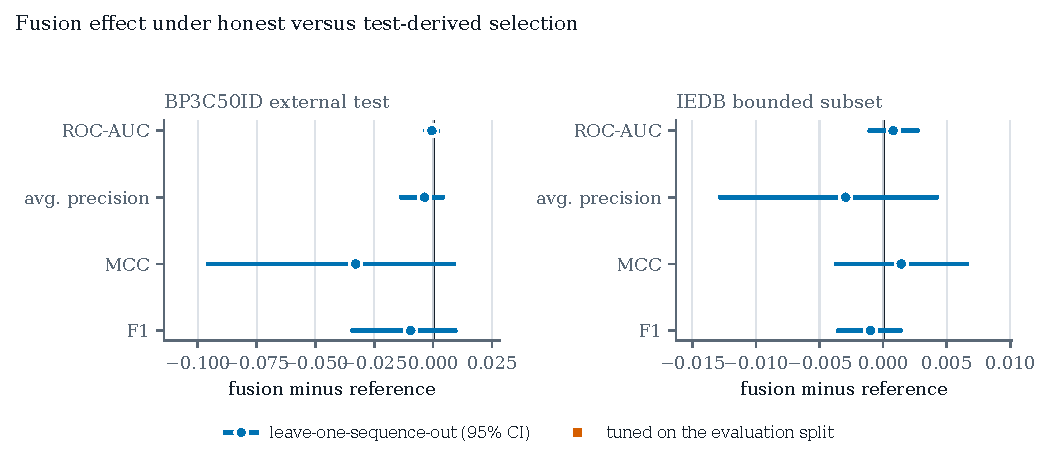
\includegraphics[width=\textwidth]{figures/fig_fusion_forest.pdf}
\caption{The fusion effect against the reference predictor under two selection
protocols. Blue intervals are mean per-antigen differences with 95\% bootstrap
intervals under leave-one-sequence-out nested selection; orange squares are the
corresponding estimates when the weight and threshold are chosen on the
evaluation split. On both datasets the nested interval contains zero while the
test-derived estimate sits above it.}
\label{fig:fusion-forest}
\end{figure*}

\begin{figure*}[t]
\centering
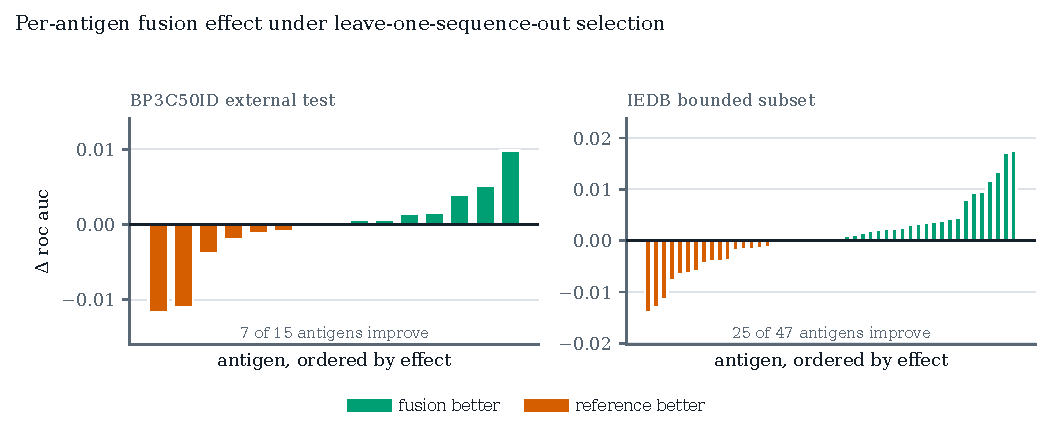
\includegraphics[width=\textwidth]{figures/fig_per_sequence.pdf}
\caption{Per-antigen change in ROC-AUC from fusion under nested selection,
ordered by effect. The dispersion, particularly on the IEDB subset, is much
larger than the mean effect in either direction.}
\label{fig:per-sequence}
\end{figure*}

Table~\ref{tab:fusion} and Figure~\ref{fig:fusion-forest} give both protocols on
both datasets.

On BP3C50ID, nested selection leaves a mean per-antigen difference against
BepiPred-3.0 of \NestedBpThreeDeltaAuc{} ROC-AUC
[\NestedBpThreeDeltaAucLo{}, \NestedBpThreeDeltaAucHi{}], with
\NestedBpThreeWinsAuc{} of \NestedBpThreeSequences{} antigens improving and a
Wilcoxon $p$ of \NestedBpThreePAuc{}. MCC behaves the same way
(\NestedBpThreeDeltaMcc{} [\NestedBpThreeDeltaMccLo{}, \NestedBpThreeDeltaMccHi{}],
$p=\NestedBpThreePMcc{}$).

The larger IEDB subset behaves the same way, with one important difference in
what it tests. We have no BepiPred-3.0 predictions for those antigens, so that
arm fuses the candidate with our own local-only predictor rather than with
BepiPred-3.0. It is a second instance of the same selection question, not a
replication of the same comparison, and we do not read it as independent
confirmation of the BepiPred-3.0 result. The mean per-antigen
difference in ROC-AUC is \NestedIedbDeltaAuc{}
[\NestedIedbDeltaAucLo{}, \NestedIedbDeltaAucHi{}], with
\NestedIedbWinsAuc{} of \NestedIedbSequences{} antigens improving
($p=\NestedIedbPAuc{}$), and MCC gives \NestedIedbDeltaMcc{}
[\NestedIedbDeltaMccLo{}, \NestedIedbDeltaMccHi{}]. Every interval on both
datasets contains zero. Both the Wilcoxon test and the sign test discard
antigens whose paired difference is exactly zero; on BP3C50ID this removes
\NestedBpThreeTiesAuc{} antigens for ROC-AUC and \NestedBpThreeTiesMcc{} for
MCC, and on the IEDB subset \NestedIedbTiesAuc{} and \NestedIedbTiesMcc{}, so
the effective sample size is smaller than the stated number of antigens by
that count.

We are careful about what these nulls support. An interval containing zero is
not evidence that the effect is zero, and at these sample sizes the paired
design cannot resolve effects of the size at issue. With the observed
per-antigen dispersion, the smallest difference BP3C50ID could detect with
80\% power at a two-sided 5\% level is \NestedBpThreeMdeMcc{} in MCC and
\NestedBpThreeMdeAuc{} in ROC-AUC; on the IEDB subset the corresponding
figures are \NestedIedbMdeMcc{} and \NestedIedbMdeAuc{}. The MCC effect the
test-derived protocol reports, \TunedBpThreeDeltaMcc{}, is far below what the
nested analysis could have detected. A non-significant nested result was close
to guaranteed, so it carries little evidential weight against that specific
effect.

What the design does identify is the behaviour of the estimator. Under the
test-derived protocol the same BP3C50ID data yield \TunedBpThreeDeltaMcc{} MCC
and \TunedBpThreeDeltaAuc{} ROC-AUC in favour of fusion; under nested
selection the same quantity on the same data is \NestedBpThreeDeltaMcc{} and
\NestedBpThreeDeltaAuc{}. The point estimate does not shrink towards zero, it
changes sign. That is a statement about how much the selection step moves the
estimate, which this comparison does identify, rather than a statement about
the underlying effect, which it does not. The defensible conclusion is that
the test-derived estimate is biased by at least the distance between the two,
not that fusion does not help.

Figure~\ref{fig:per-sequence} shows the per-antigen differences behind these
means. The dispersion is far larger than the mean in both directions. That is
what a null effect over a small number of antigens looks like, and it is the
reason we report the paired tests rather than a pooled number alone.

\subsection{How often the published literature selects this way}
\label{sec:survey}

The result above is a correction to our own unpublished analysis, which bounds
how much it matters. To ask whether the practice is confined to us, we
surveyed published B-cell epitope predictors that combine two or more models
--- score fusion, ensembles, stacking, consensus voting --- and asked of each
whether the combination parameter was chosen using the same data the headline
performance is reported on. The survey covers
\SurveyAssessed{} assessable papers and records, for every one, the verbatim
sentence the judgement rests on; it is released with the code.

We keep three categories apart. \SurveyLeakage{} papers are \emph{leakage
evident}: the text states that a mixing weight, a voting rule, an ensemble
composition or a reported configuration was chosen by inspecting performance
on the evaluation data. \SurveyClean{} are \emph{leakage-free evident}: a
validation split, the training set, or a rule fixed a priori.
\SurveyUnreported{} are \emph{unreported}: the paper does not say on which
data the parameter was chosen. We do not count the third group as leakage. It
is an observation about what the methods section contains, and its size is
itself the point --- a quarter of the sample does not let a reader check.
Among the \SurveyStatingBasis{} papers that do state a basis,
\SurveyLeakageShare{}\% selected on their own evaluation data.

These counts are not a prevalence estimate and we do not offer them as one.
The sample is open-access only, reachable by keyword, and skewed towards
recent and prominent work; paywalled methods papers are structurally absent.
With \SurveyAssessed{} papers each count carries a sampling error of one or
two. What the survey does establish is that the selection step we found in our
own work is present in the published literature, that it is not rare among
papers that disclose enough to tell, and that a substantial minority of papers
disclose too little for the question to be asked at all. The magnitude such a
step can reach is the subject of the next section.

\subsection{How large the selection step is, and what governs it}
\label{sec:bias-curve}

The sections above establish that the selection step moved our estimate and
that the practice occurs in print. Neither says how large an effect a reader
should expect it to produce. That is answerable from the same data by
resampling.

For a given antigen count and weight grid we draw a subset without
replacement, estimate the fused-minus-reference difference on it twice, and
record the gap. The first estimate scans the grid on the subset and keeps the
best row, which is the protocol a paper follows when it reports a tuned
combination parameter without holding anything out. The second applies
leave-one-sequence-out selection inside the same subset. Both estimators see
exactly the same antigens, so the gap is attributable to the selection rule
rather than to which data were drawn. We average over \BiasReplicates{} draws
per cell.

\begin{figure*}[t]
\centering
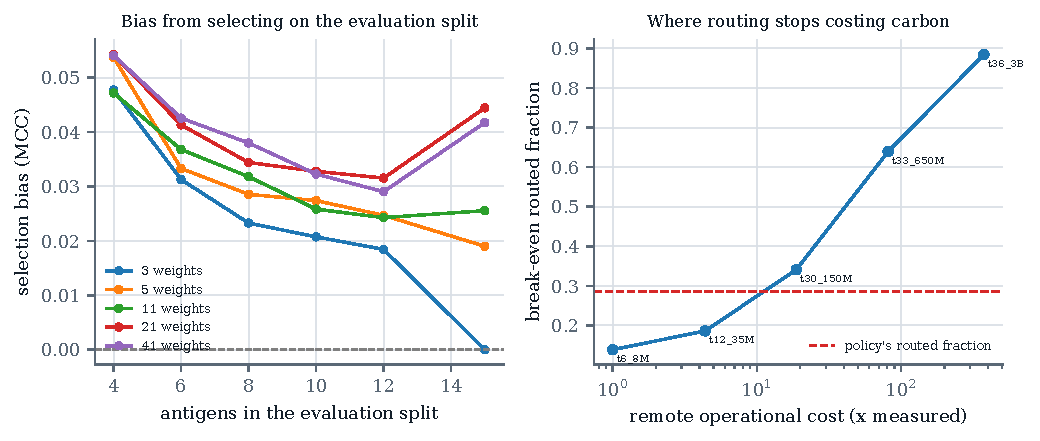
\includegraphics[width=\textwidth]{figures/fig_selection_bias.pdf}
\caption{Left: the mean gap between a weight chosen on the evaluation split
and one chosen by leave-one-sequence-out selection within it, over
\BiasReplicates{} draws per cell, by antigen count and weight-grid density.
Both estimators see the same antigens in every draw. The rightmost point of
each series is the full split, where only one subset exists; it is a single
deterministic run rather than a mean, which is why the coarsest grid reaches
exactly zero there, and it should not be read as part of the trend. Right:
the break-even routed fraction of
Equation~\ref{eq:carbon-threshold} as the remote tier is scaled, with the
policy's own routed fraction marked. The released ESM-2 checkpoints are
labelled; the ordering reverses between \(35\)M and \(150\)M. Both panels
are modelled from the recorded constants, not metered.}
\label{fig:selection-bias}
\end{figure*}

The bias is positive everywhere and large relative to the effects this
literature reports (Figure~\ref{fig:selection-bias}, left). On \BiasMetric{}
it runs from \BiasAtSmallestN{} at
\BiasSmallestN{} antigens to \BiasAtLargestN{} at \BiasLargestN{}. It grows
with the density of the grid: at \BiasGridRefN{} antigens a
\BiasCoarseGridPoints{}-point grid yields \BiasCoarseGridBias{} and a
\BiasFineGridPoints{}-point grid \BiasFineGridBias{}, which is what one would
expect if a finer scan simply offers more chances to fit the evaluation split.
At the grid densities ordinarily used --- weight steps of \(0.05\) are
common --- the test-derived estimate was the more favourable one in
\BiasPositiveShareLargestN{}\% of draws. The full-split cell reproduces the
headline of Section~\ref{sec:fusion-results} exactly, at
\BiasAtLargestN{}, which is the difference between the
\TunedBpThreeDeltaMcc{} that protocol reports and the
\NestedBpThreeDeltaMcc{} nested selection returns.

The comparison worth drawing is between that bias and the effects it is used
to support. Our own earlier analysis reported a gain of
\TunedBpThreeDeltaMcc{} \BiasMetric{}. The expected bias at that sample size
and grid density is several times larger. A tuned fusion result of that
magnitude, on a benchmark of this size, therefore carries no information about
whether fusion helps: it is within what the selection rule alone produces.
This is the sense in which the present work generalises beyond one corrected
analysis. The bias is not an accident of our predictors; it is a property of
scanning a grid on a small evaluation set, and its size can be estimated in
advance for any such design.

We are careful about the scope. These magnitudes are specific to these two
predictors, whose mean rank agreement across cells is \BiasAgreement{}; two
predictors that agree less would leave more room for a scan to exploit, and
two that agree more would leave less. What transfers is the construction and
the direction, not the numbers.

\subsection{Which predictor the procedure prefers}
\label{sec:weight-transfer}

\begin{figure*}[t]
\centering
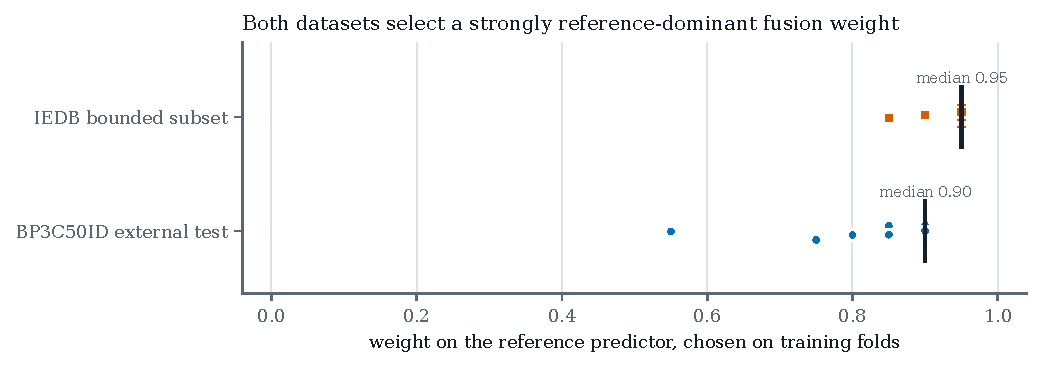
\includegraphics[width=\textwidth]{figures/fig_weight_stability.pdf}
\caption{The fusion weight selected in each training fold, by dataset, with
medians marked. Both datasets place almost all of the weight on the reference
predictor, which is the same conclusion the null effect reaches by a different
route.}
\label{fig:weight-stability}
\end{figure*}

Figure~\ref{fig:weight-stability} plots the weight chosen in each training fold.
On BP3C50ID the folds settle around a median of \NestedBpThreeWeightMedian{}
(range \NestedBpThreeWeightMin{} to \NestedBpThreeWeightMax{}); on the IEDB
subset the median is \NestedIedbWeightMedian{} (range \NestedIedbWeightMin{} to
\NestedIedbWeightMax{}). Both sit close to the upper end of the grid, meaning
the selection procedure chooses to give our predictor almost no influence over
the blended score.

The selected weights are an independent route to the same
conclusion. The nested evaluation says the blend cannot be distinguished from
the reference predictor. The selected weights say why: the
procedure, given a free choice, declines to use the second predictor. A fusion
whose fitted weight approaches one is not a combination of two models but the
stronger model with extra machinery attached.
